\section{Simultaneous position/force control}\label{sec:pos-force-control-exp}

\begin{table}[]
    \centering
    \begin{tabular}{|c|c|c|}
        \hline
        & Value & Unit\\
        \hline
        Number of obstacles & $3$ & \\
        Number of links & $6$ & \\
        $f_{F,d,3}$ & $1$ & $N$ \\
        $\theta_{t,d,3}$ & $0.1$ & $rad$ \\
        Force:$[K_{p}, K_{i}]$ & $[1, 0.005]$ &\\
        Position:$[K_{p}, K_{i}]$ & $[3, 0.005]$ &\\
        \hline
    \end{tabular}
    \caption{Simulation configuration for force control experiment with minimal CKCs}
    \label{tab:p+f}
\end{table}

\begin{figure}
    \centering
    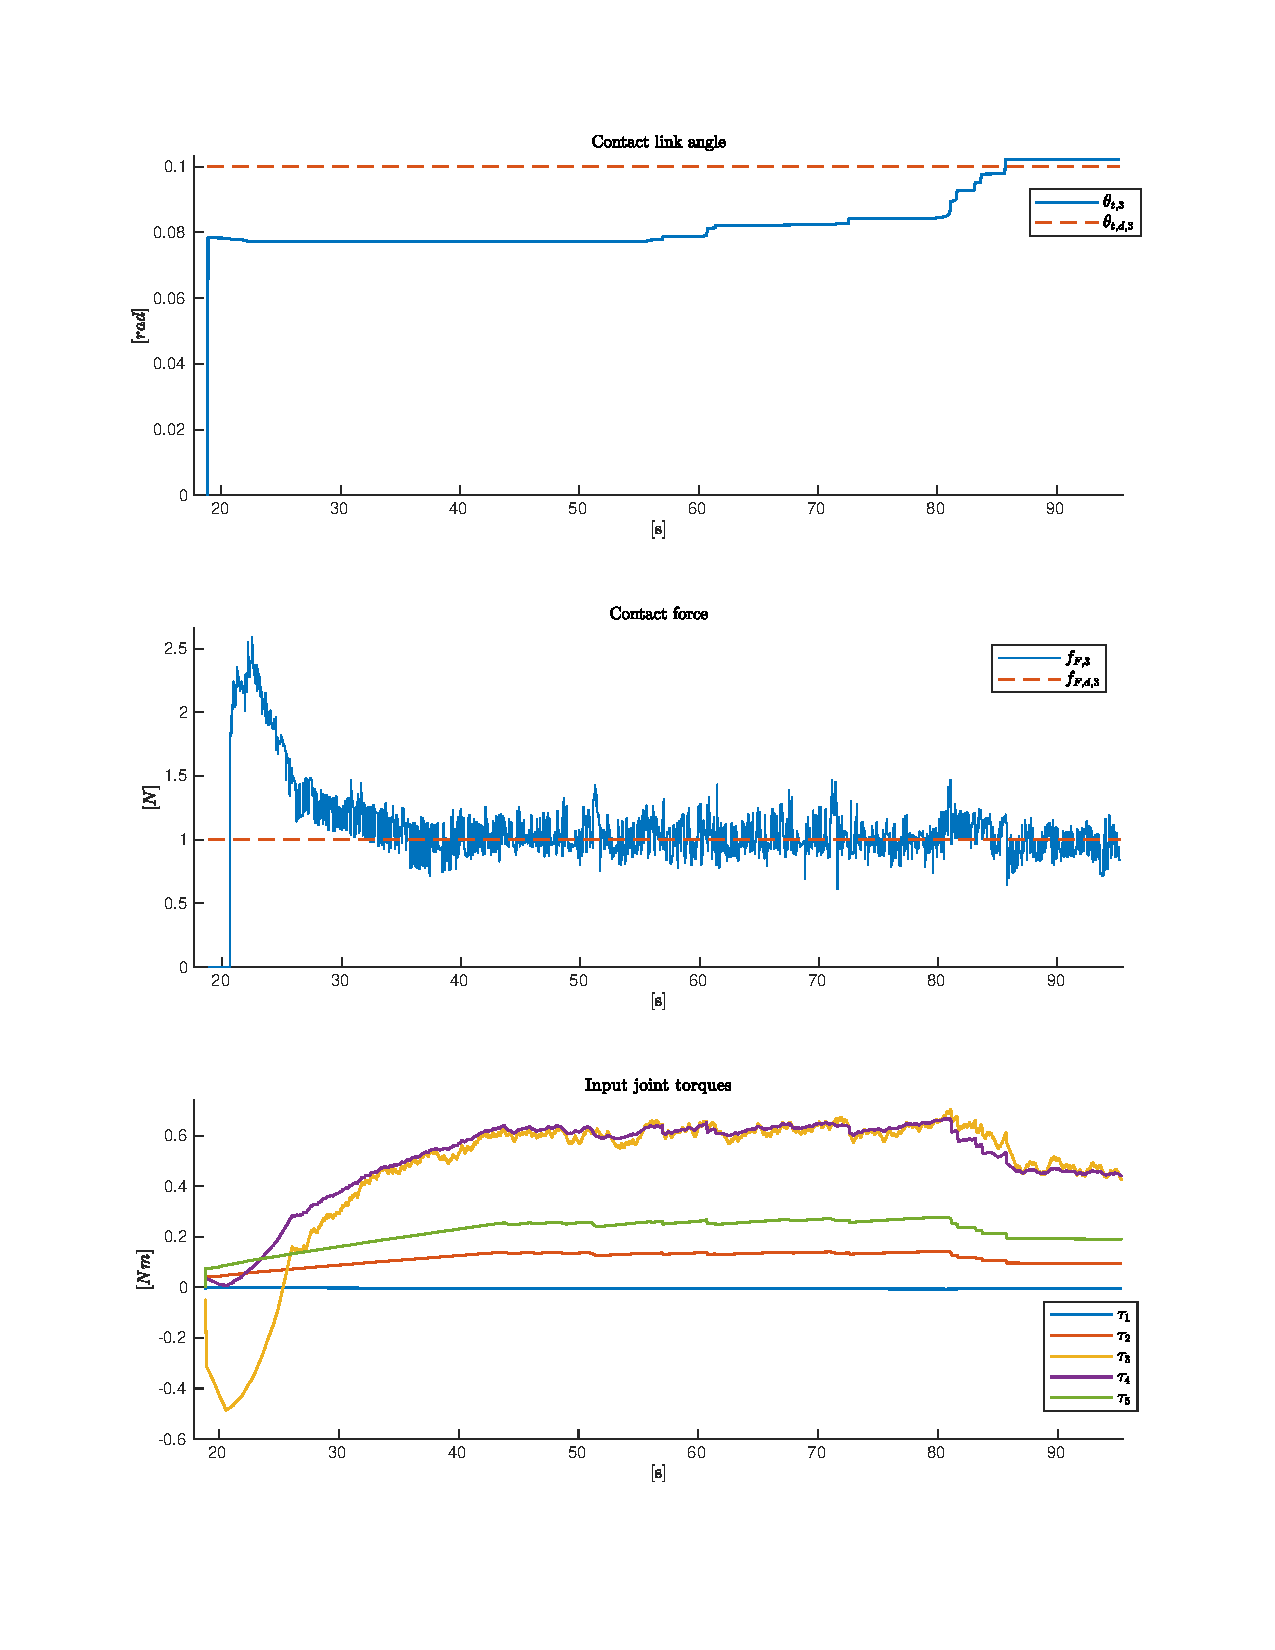
\includegraphics[trim=2.1cm 2.1cm 2.1cm 2.1cm, clip=true, width=\textwidth]{figures/experiments/pos+f/pf-ref-3.pdf}
    \caption{Simultaneous force and position control}
    \label{fig:p+f}
\end{figure}